\subsection{Evolúciós algoritmusok, evolúció stratégiák, genetikus programozás.}

\textbf{Evolúciós algoritmusok:}
\begin{itemize}
    \item alapelvük a megoldások egy populációján történő keresés, melyet a biológiából megismert törvényszerűségek vezérelnek
    \item gén: funkcionális entitás, ez egyed egy speciális tulajdonságát kódolja (pl. hajszín)
    \item allél: a gén értéke (pl. szőke)
    \item egyed: kromoszóma, egy megoldás jelölt a problémára
    \begin{itemize}
        \item a probléma egy lehetséges megoldása valamilyen formában az egyedbe van kódolva (pl. bináris, vagy valós)
        \item fitnesz érték: az egyedeket valamilyen kritérium szerint kiértékeljük, aszerint, hogy milyen jó megoldást adnak a problémára
        \item jobb egyedeknek nagyobb a fitnesz értéke, nagyobb eséllyel élnek túl
    \end{itemize}
    \item genotípus: egy egyed alléljainak egy speciális kombinációja
    \item fenotípus: egy egyed külső-belső tulajdonságainak összessége
    \item locus: egy gén pozíciója a kromoszómán belül
    \item populáció: egyszerre együtt élő egyedek összessége
    \begin{itemize}
        \item fejlődik, egyre jobb egyedeket kapunk
    \end{itemize}
    \begin{center}
        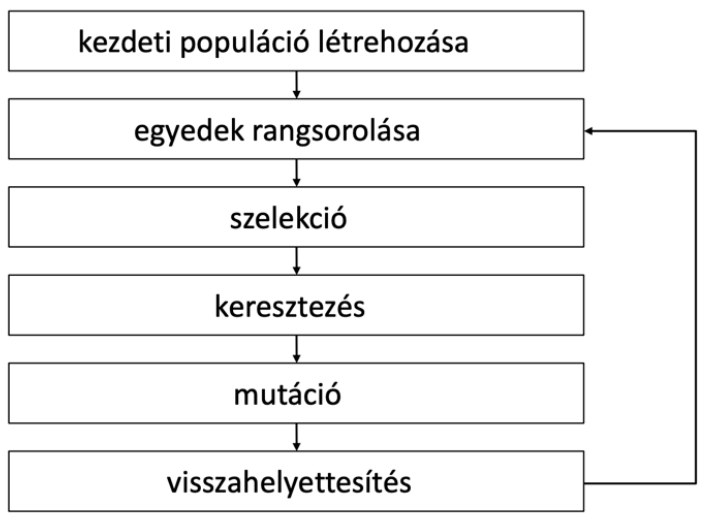
\includegraphics[width=0.6\textwidth]{res/imgs/info_27_evolutionary_algorithm.png}
    \end{center}
    \item szelekciós módszerek:
    \begin{itemize}
        \item minél jobb az egyed, annál nagyobb az esély a kiválasztásra
        \item \begin{minipage}[t]{0.5\textwidth} rulett kerék szelekció: az egyedek a fitnesz értékükkel arányos nagyságú szeletet kapnak \end{minipage} \begin{minipage}[t]{0.4\textwidth} \vspace{-15pt} \begin{center} 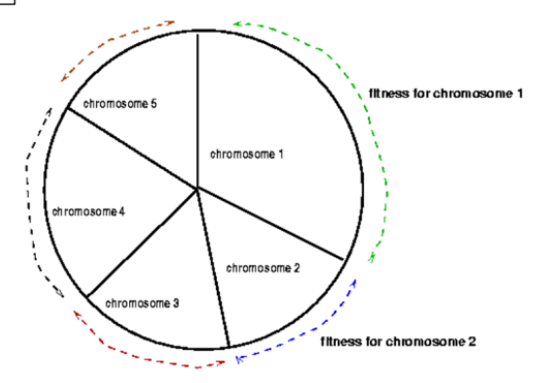
\includegraphics[width=\textwidth]{res/imgs/info_27_roulette_selection.png} \end{center} \end{minipage}
    \end{itemize}
    \vspace{10pt}
    \item keresztezés:
    \begin{itemize}
        \item véletlenszerű keresztezési pont kiválasztása két szülőn
        \item utódok létrehozása az információ kicserélődésével a keresztezési pont alapján
    \end{itemize}
    \begin{center}
        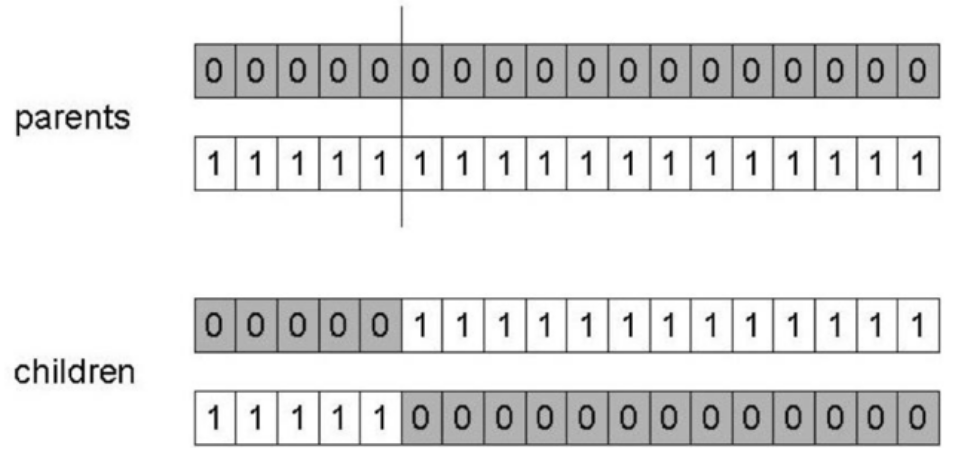
\includegraphics[width=0.7\textwidth]{res/imgs/info_27_crossover.png}
    \end{center}
    \item mutáció:
    \begin{itemize}
        \item gén értékének véletlenszerű megváltoztatása $p_m$ valószínűséggel (mutációs arány)
    \end{itemize}
    \begin{center}
        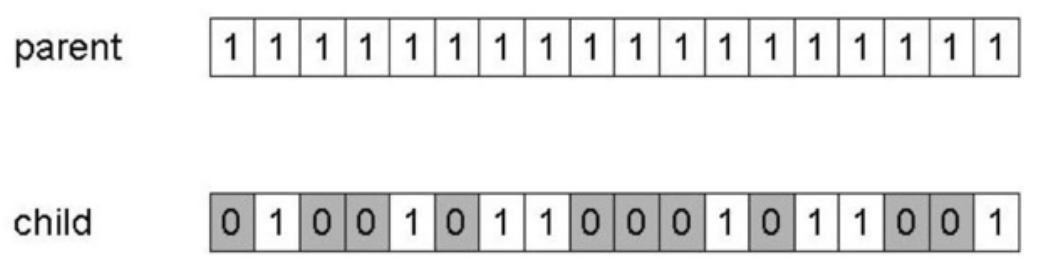
\includegraphics[width=0.7\textwidth]{res/imgs/info_27_mutation.png}
    \end{center}
\end{itemize}

\textbf{Genetikus programozás:}
\begin{itemize}
    \item genetikus algoritmusok alapötletét alkalmazza
    \item különböző problémák, különböző területekről átfogalmazhatók egy számítógépes program-keresési feladattá
    \begin{center}
        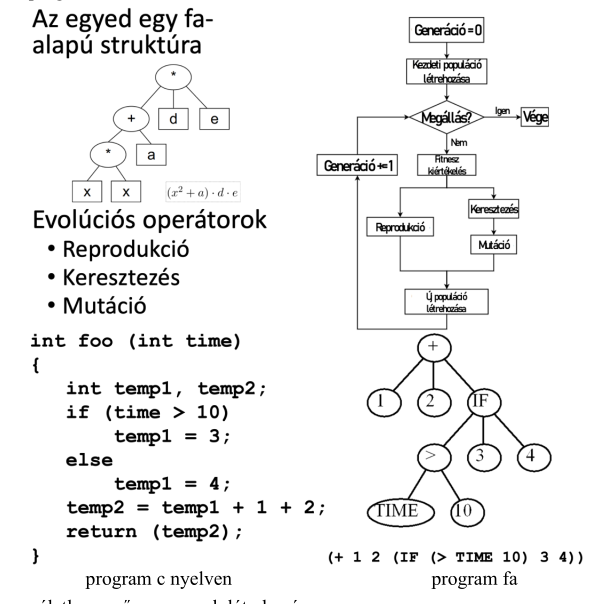
\includegraphics[width=0.95\textwidth]{res/imgs/info_27_genetic_programming.png}
    \end{center}
    \item véletlenszerű programok létrehozása:
    \begin{itemize}
        \item rendelkezésre álló függvények: pl. $F = \{+, -, *, /, IF\}$
        \item rendelkezésre álló terminálisok: pl. $T = \{X, Y, \text{konstansok}\}$
        \item véletlen programok:
        \begin{itemize}
            \item szintaktikailag érvényesek
            \item végrehajthatók
        \end{itemize}
        \item a fák különböző méretűek és alakúak lehetnek
    \end{itemize}
    \item genetikus operátorok:
    \begin{itemize}
        \item reprodukció:
        \begin{itemize}
            \item szülő kiválasztása (fitnesz alapján)
            \item változatlan lemásolása a populáció következő generációjába
        \end{itemize}
        \item mutáció:
        \begin{itemize}
            \item 1 szülő kiválasztása (fitnesz alapján)
            \item a fa egy pontjának kiválasztása
            \item a kiválasztott pontnál lévő részfa törlése
            \item új részfa növesztése a mutációs pontnál (véletlen fa létrehozása)
            \item az eredmény szintaktikailag érvényes és végrehajtható program legyen
            \item leszármazott elhelyezése a populáció következő generációjába
        \end{itemize}
        \begin{center}
            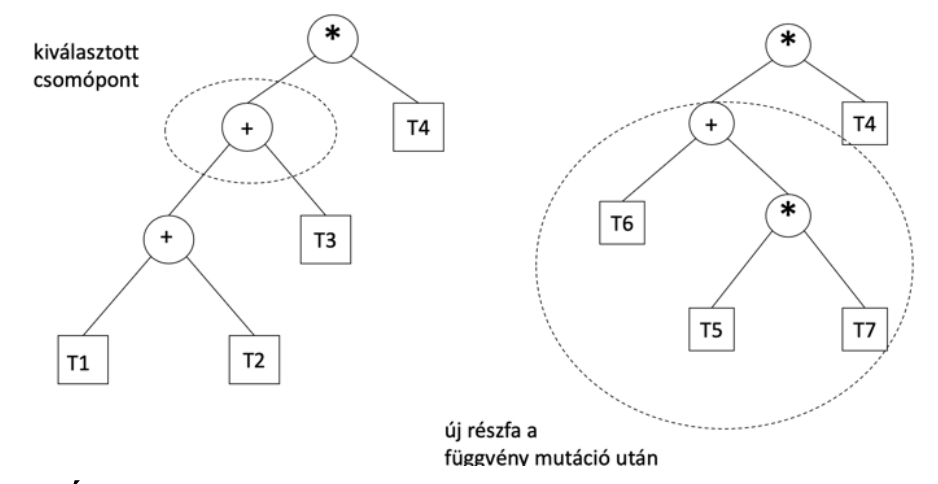
\includegraphics[width=0.8\textwidth]{res/imgs/info_27_subtree_mutation.png}
        \end{center}
        \item keresztezés:
        \begin{itemize}
            \item 2 szülő kiválasztása (fitnesz érték alapján)
            \item első szülő fájában egy véletlen pont kiválasztása
            \item második szülő fájában egy véletlen pont kiválasztása
            \item a két kiválasztott ponthoz tartozó részfák kicserélése
            \item az eredmények szintaktikailag érvényes és végrehajtható programok legyenek
            \item leszármazottak elhelyezése a populáció következő generációjába
        \end{itemize}
    \end{itemize}
    \item előkészítő lépések:
    \begin{itemize}
        \item a terminálisok halmazának meghatározása
        \item függvények halmazának meghatározása
        \item fitnesz mérték meghatározása
        \item futtatás paramétereinek meghatározása
        \item megállási feltétel meghatározása
    \end{itemize}
\end{itemize}